%!TEX root = ../ap_gcc.tex

\section{Tutorial}
\label{sec:Tutorial}

This section shows how to profile a project step by step. In general, the process is quite similar to the process needed to profile a project with the Windows version of callmon. Big differences only appear in the build configuration due to differences in the compiler switches needed by GCC.

In this tutorial, we use ioQuake3 profiling on Mac OS X as a sample, but for other projects, the process stays the same.

\subsection{Preparing the build process} How to prepare the build process.

\subsubsection{Parameters to GCC} This is a list of parameters needed by GCC when profiling with unix fact extraction.

\paragraph{Compile with -g} Enable debug information.

With this option enabled, GCC builds debug information into the resulting binary. This is needed by metacreator to resolve source file name, line numbers and other valuable debugging information.

Note that you can still compile with optimizations enabled (\inlinecode{-O2} and friends) since our mechanism finds multiple enters and exists per function.

\paragraph{Compile with -finstrument-functions} Enable instrumentation.

This GCC parameter is the key. With this option enabled, GCC inserts calls to instrumentation functions right after a function was called and right before a function returns. If you do not provide this option in the compilation process, no calls will be made to the unix callmon library, and therefor no profiling information can be retrieved.

\paragraph{Compile with -fno-inline} Disable inlining of functions.

This disables the inlining of functions which is done explicitly by the developer or automatically by the compiler to optimize execution speed by eliminating function call overhead.

Since we are profiling on a function execution level, we cannot profile inlined function, so all the functions inlined by the compiler cannot appear in the call graph. To be sure this cannot happen, use \inlinecode{-fno-inline} as a GCC option. You might skip this if you want. You still might get good profiling results for the calls you are interested in, but you have been warned!

\paragraph{Link unixcallmon library as the last library} Ensure the right profiling functions are used.

It might happen, that other libraries as well provide the profiling functions that unix callmon lib provides (glib is an example for that). If this happens, it is important to ensure that the versions of the unix callmon lib are the ones linked in. This is done by adding the \inlinecode{-lunixcallmon\_lib} parameter as the last one.

\paragraph{On Linux, link with -Wl,-Bsymbolic} Make function calls patchable.

\todo{explain this case more in detail, just happens with .so s, etc.}

Without this option, symbolic function call information is removed from the resulting binary on Linux. This prevents \toolname{cga\_patch} and \toolname{cga\_patchclean} from finding the call locations and makes it impossible to remove those calls from the binary. 

\paragraph{Build with absolute path to source} Ensure CGA can find source files.

To ensure that CGA can find the source files for the source code viewer, you need to provide GCC with the absolute path to the source file while compiling.

\subsubsection{Putting it all together} If the project you want to analyze is build using make, you might want to add the following to the projects Makefile:

\begin{verbatim}
  CFLAG   += -g -finstrument-functions -fno-inline 
  CXXFLAG += -g -finstrument-functions -fno-inline 
  LDFLAGS += -Wl,-Bsymbolic -L/path/to/callmonlib -lunixcallmon_lib
\end{verbatim}

For ioQuake3, we added the following in \pathname{IOQUAKE3\_ROOT/Makefile} in the \inlinecode{ifeq (\$(PLATFORM),darwin)} section (around line 360):

\begin{verbatim}
  BASE_CFLAGS  = -Wall -Wimplicit -Wstrict-prototypes
  BASE_CFLAGS += -fno-inline
  BASE_CFLAGS += -finstrument-functions 
  LDFLAGS     += -L/path/to/callmonlib -lunixcallmon_lib -lstdc++
\end{verbatim}

\subsection{Building the application} With all the above mentioned set up, you build your project as usual, e.g. by typing \toolname{make}.

The ioQuake3 has a special target named \inlinecode{debug}, so you need to type \inlinecode{make debug} to include debugging symbols in the executable.

\subsection{Patching the executable} To enable the following command lines to work you might have to move the executables \toolname{cga\_patchclean} \toolname{cga\_patch}, \toolname{cgatoolbar} and \toolname{metacreator} to some location in your \inlinecode{PATH} or symlink them accordingly.

As soon as the build process has finished, you end up with an executable or library which has all the profiling mechanisms build in. At this point, every single function which was just compiled by GCC is now enriched by profiling logic. Since this may be a lot, you might want to exclude several functions or groups of functions from the profiling process. This is done by patching the binary. Technically, the calls to the instrumentation functions get overwritten by NOP operations, so almost no overhead is involved in calling functions removed from the profiling process.

\subsubsection{Patch clean} The first thing to do is call \toolname{cga\_patchclean} on the binary like this:
\begin{verbatim}
  $ cd build/debug-darwin-i386
  $ cga_patchclean ioquake3.i386 ioquake3.i386.patch
\end{verbatim}
The first parameter specifies the binary to patch. The second parameter specifies a patch file name. In this patch file, \toolname{cga\_patchclean} will write out all the locations from which profiling calls were removed along with the opcodes removed that realized the call. This information is needed by \toolname{cga\_patch} to re-include the call opcodes for certain functions in the next step.

\subsubsection{Patch} At this point, profiling logic is re-added to the functions of interest. This is done by specifying two groups of function name patterns in a pattern file. This is exactly the same like for Windows callmon.

Provide a list of patterns in the include section, as well a list of patterns in the exclude section. Then, call patch like this:

\begin{verbatim}
  $ cga_patch ioquake3.i386 ioquake3.i386.patch myPatternsFile.txt
\end{verbatim}

You may leave the patterns file parameter empty to re-include all functions in the profiling process. Like this:

\begin{verbatim}
  $ cga_patch ioquake3.i386 ioquake3.i386.patch
\end{verbatim}

\subsection{Using CGA Toolbar}

The CGA Toolbar can be used as usual. It needs to set up the environment variable \inlinecode{CALLMON\_HOME}. This variable has to contain the path, where the log files are created. So lets say, you have a directory structure like this:

\begin{verbatim}
  <working directory>/
  |
  |- ioquake3.i386
  |- ioquake3.i386.patch
  |- myPatternsFile.txt
\end{verbatim}

Create a directory where the CGA Toolbar can operate on, like this:

\begin{verbatim}
  $ mkdir -p logs/ioquake3.i386
\end{verbatim}

You end up with a directory structure like this:

\begin{verbatim}
  <working directory>/
  |
  |- logs/
  |  |
  |  |- ioquake3.i386/
  |     |
  |     |
  |
  |- ioquake3.i386
  |- ioquake3.i386.patch
  |- myPatternsFile.txt
\end{verbatim}

Now, fire up the CGA Toolbar like this:

\begin{verbatim}
  $ CALLMON_HOME="<working directory>" cgatoolbar
\end{verbatim}

The string \emph{ioquake3} should now show up in the drop down menu in the CGA Toolbar. If you now hit the start button, CGA Toolbar will create a file called \pathname{callmon.cmd}:

\begin{verbatim}
  <working directory>/
  |
  |- logs/
  |  |
  |  |- ioquake3.i386/
  |     |
  |     |- callmon.cmd
  |
  |- ioquake3.i386
  |- ioquake3.i386.patch
  |- myPatternsFile.txt
\end{verbatim}

This tells callmon to log function calls. Hitting the stop button will remove this file. You are now ready to run your application and record profiling information.

\subsection{Running the application}

Run the application as usual for example like this:

\begin{verbatim}
  $ ./ioquake3.i386
\end{verbatim}

If you now press start and stop on the CGA Toolbar, new traces will be generated. Each trace will reside in the \pathname{logs/ioquake3.i386/} directory. Each trace will be put into its own directory depending on the date and time the logging started at. So after you created several traces, you might end up with a directory structure like this:   

\begin{verbatim}
  <working directory>/
  |
  |- logs/
  |  |
  |  |- ioquake3.i386/
  |     |
  |     |- callmon.cmd
  |     |- 090229_143523
  |     |- 090229_143542
  |     |- 090229_143559
  |     |- 090229_143614
  |
  |- ioquake3.i386
  |- ioquake3.i386.patch
  |- myPatternsFile.txt
\end{verbatim}

Each trace directory now contains .cmlog files, each of them representing the events that occured in one thread and .modinfo files, that contain the dynamic library state when logging started and as well when logging ended. So the directory for one trace may look like this: 

\begin{verbatim}
  090229_143542/
  |
  |-profile_4243_b8bfa41d.cmlog
  |-profile_4243_b8bfd411.cmlog
  |-profile_4243_b1ad00d2.cmlog
  |-profile_4243_pre.modinfo
  |-profile_4243_post.modinfo
\end{verbatim}

The first number in the .cmlog filename describes the process identifier, the second number in hexadecimal describes the thread identifier. The .modinfo filenames as well contain the process identifier.

\subsection{Using Metacreator}

The next step is to enrich the collected information by running \toolname{metacreator}. Do do this, you simple fire up \toolname{metacreator} and provide it with a traces directory as parameter, like this:

\begin{verbatim}
  $ metacreator ./logs/ioquake3.i386/090229_143542
\end{verbatim}

Depending on the amount of events you collected, metacreator will take some time now. For all the logged calls, metacreator will now resolve debugging information from the binary. Once finished, a new .callmon file was created in the traces directory. So it should look like this now:

\begin{verbatim}
  090229_143542/
  |
  |-profile_4243_b8bfa41d.cmlog
  |-profile_4243_b8bfd411.cmlog
  |-profile_4243_b1ad00d2.cmlog
  |-profile_4243_pre.modinfo
  |-profile_4243_post.modinfo
  |-profile_4243.callmon
\end{verbatim}

All the preparations are done now. You can now start up CGA and load the trace.

\subsection{Loading the trace(s) into CGA} Start the CGA executable, create a new project. Then, select manage traces, click the add button, select your .callmon file and let CGA import the trace.

\begin{figure}[ht]
\centering
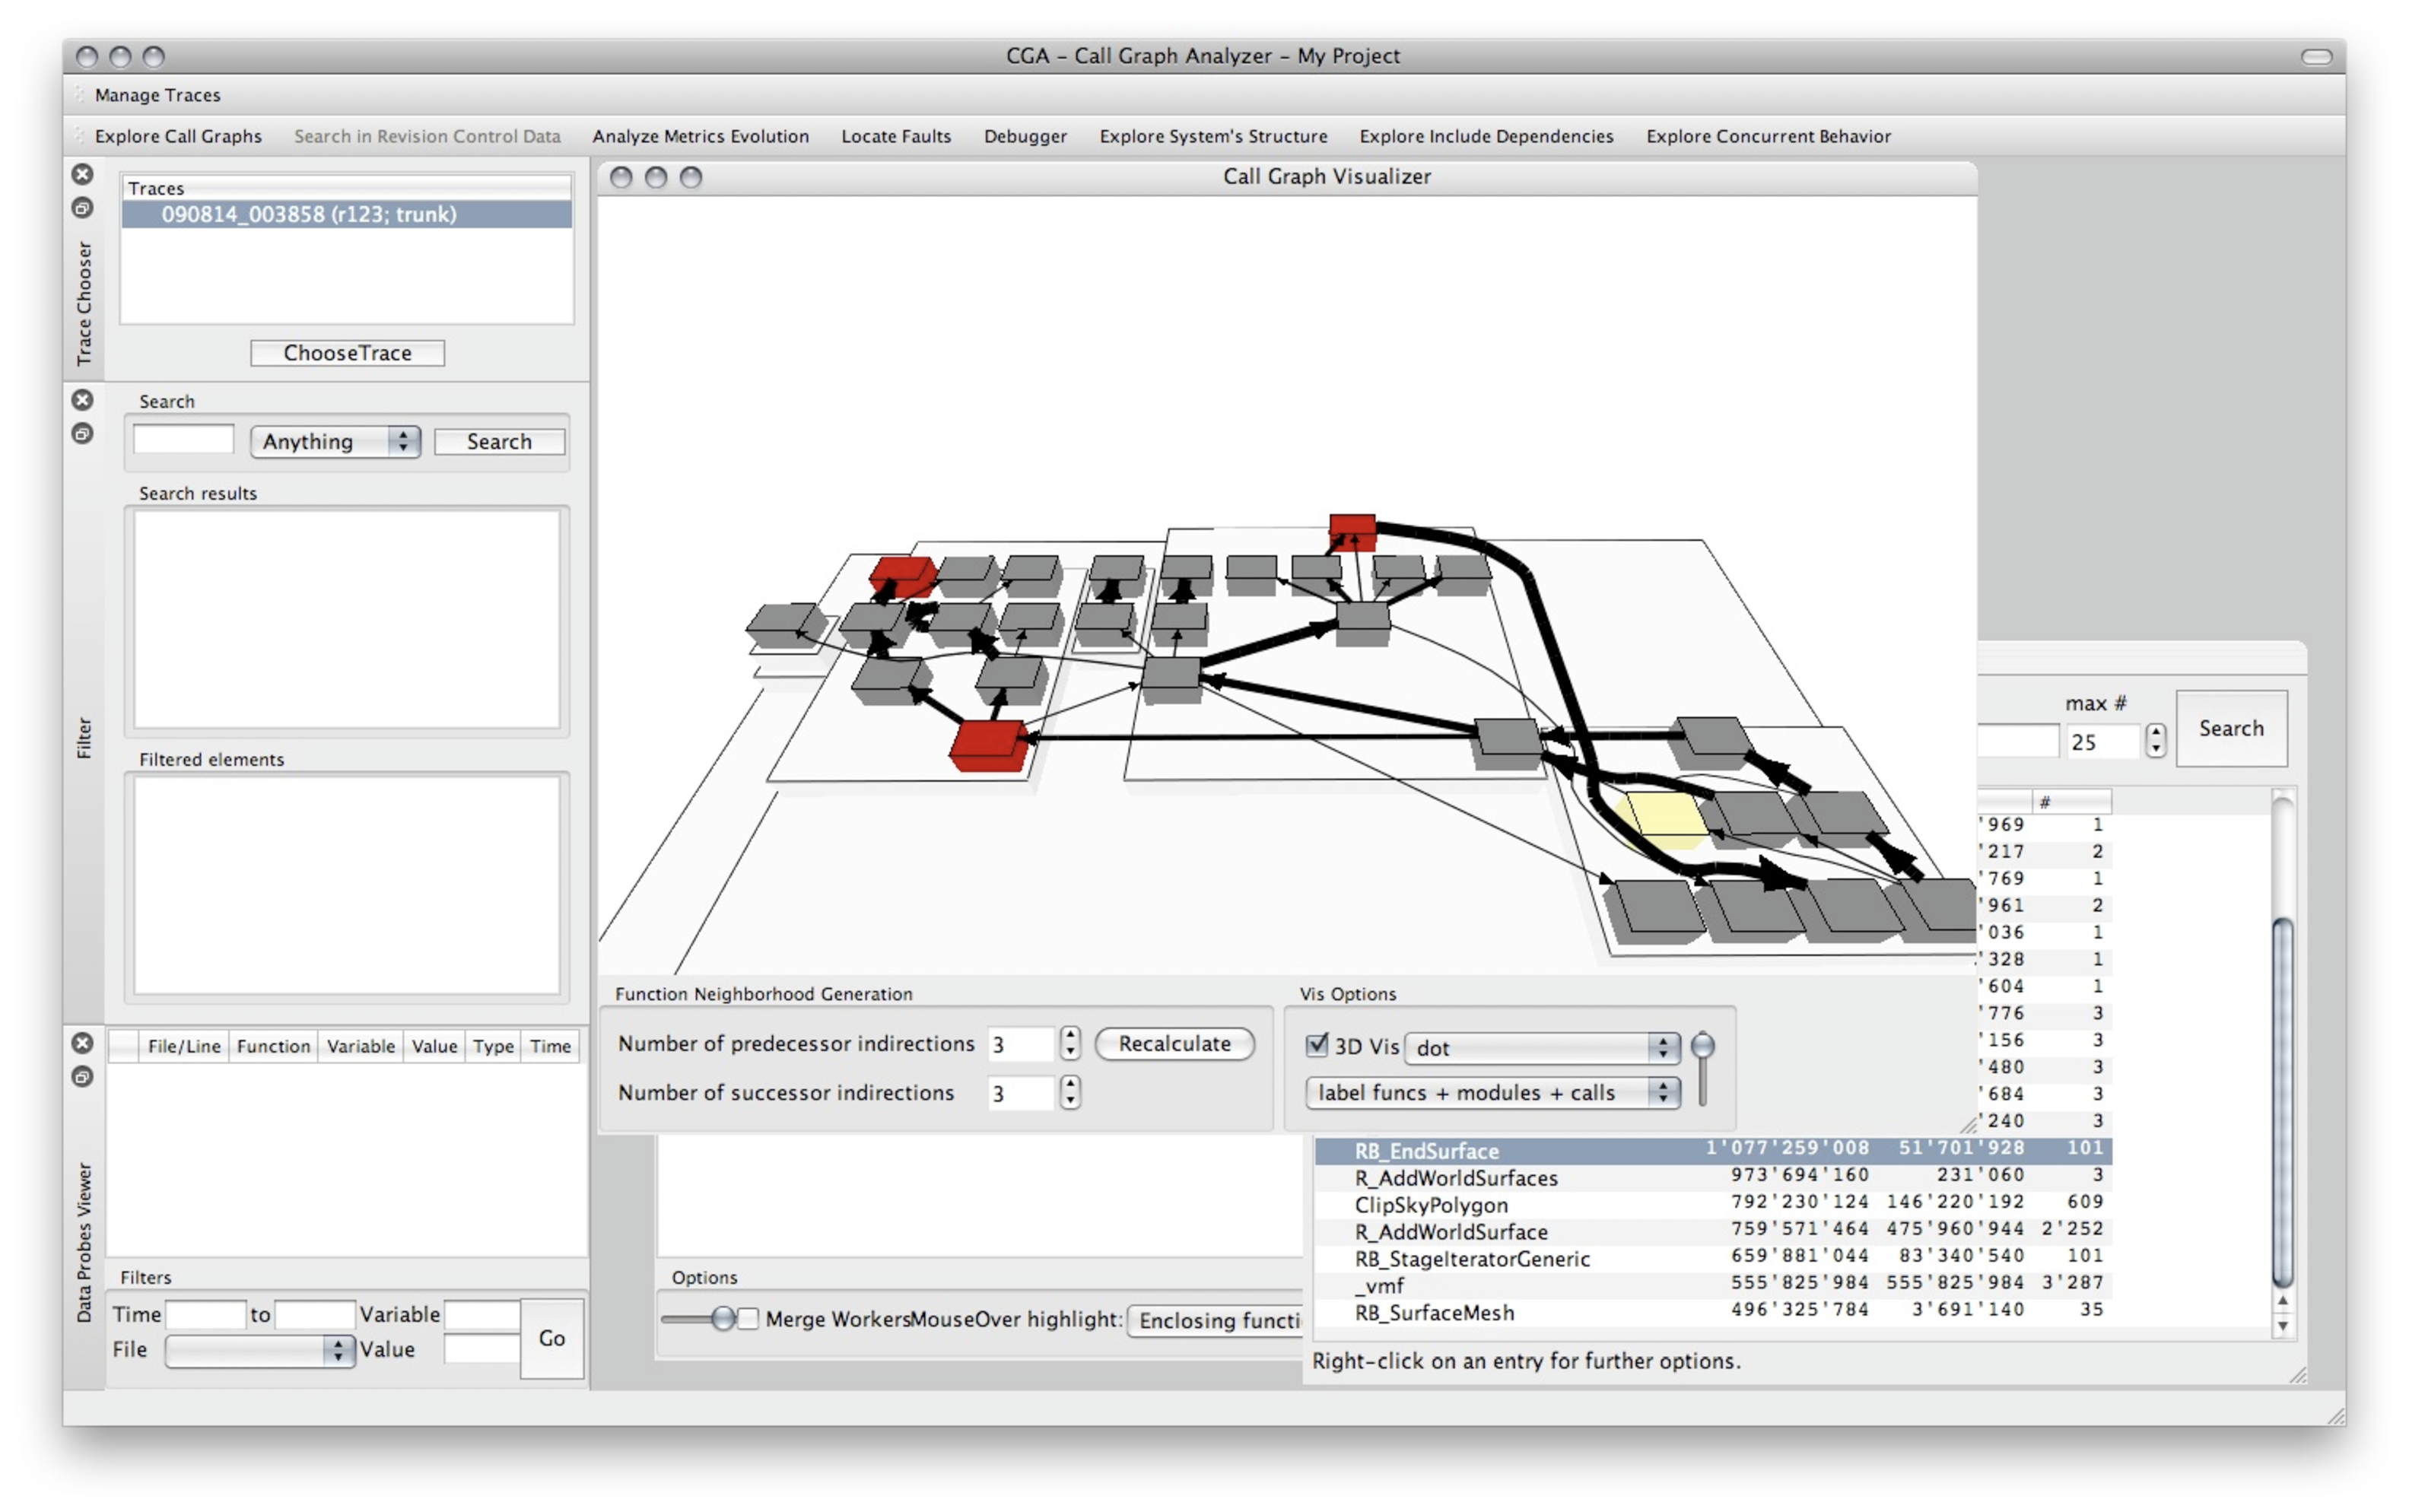
\includegraphics[width=16cm]{images/ioquake3_trace}
\caption{Trace Visualisation for ioQuake3}\label{fig:ioquake3_trace}
\end{figure}

\subsection{Multithreaded example} To show the multithreading capabilities of our system, we provide a small sample called \toolname{unixcallmontest}. This executable will be created by the CMake build process. All the special GCC flags are already set up for you. You only need to patch and profile the program as described above.

Here is how it might look like:
\begin{figure}[ht]
\centering
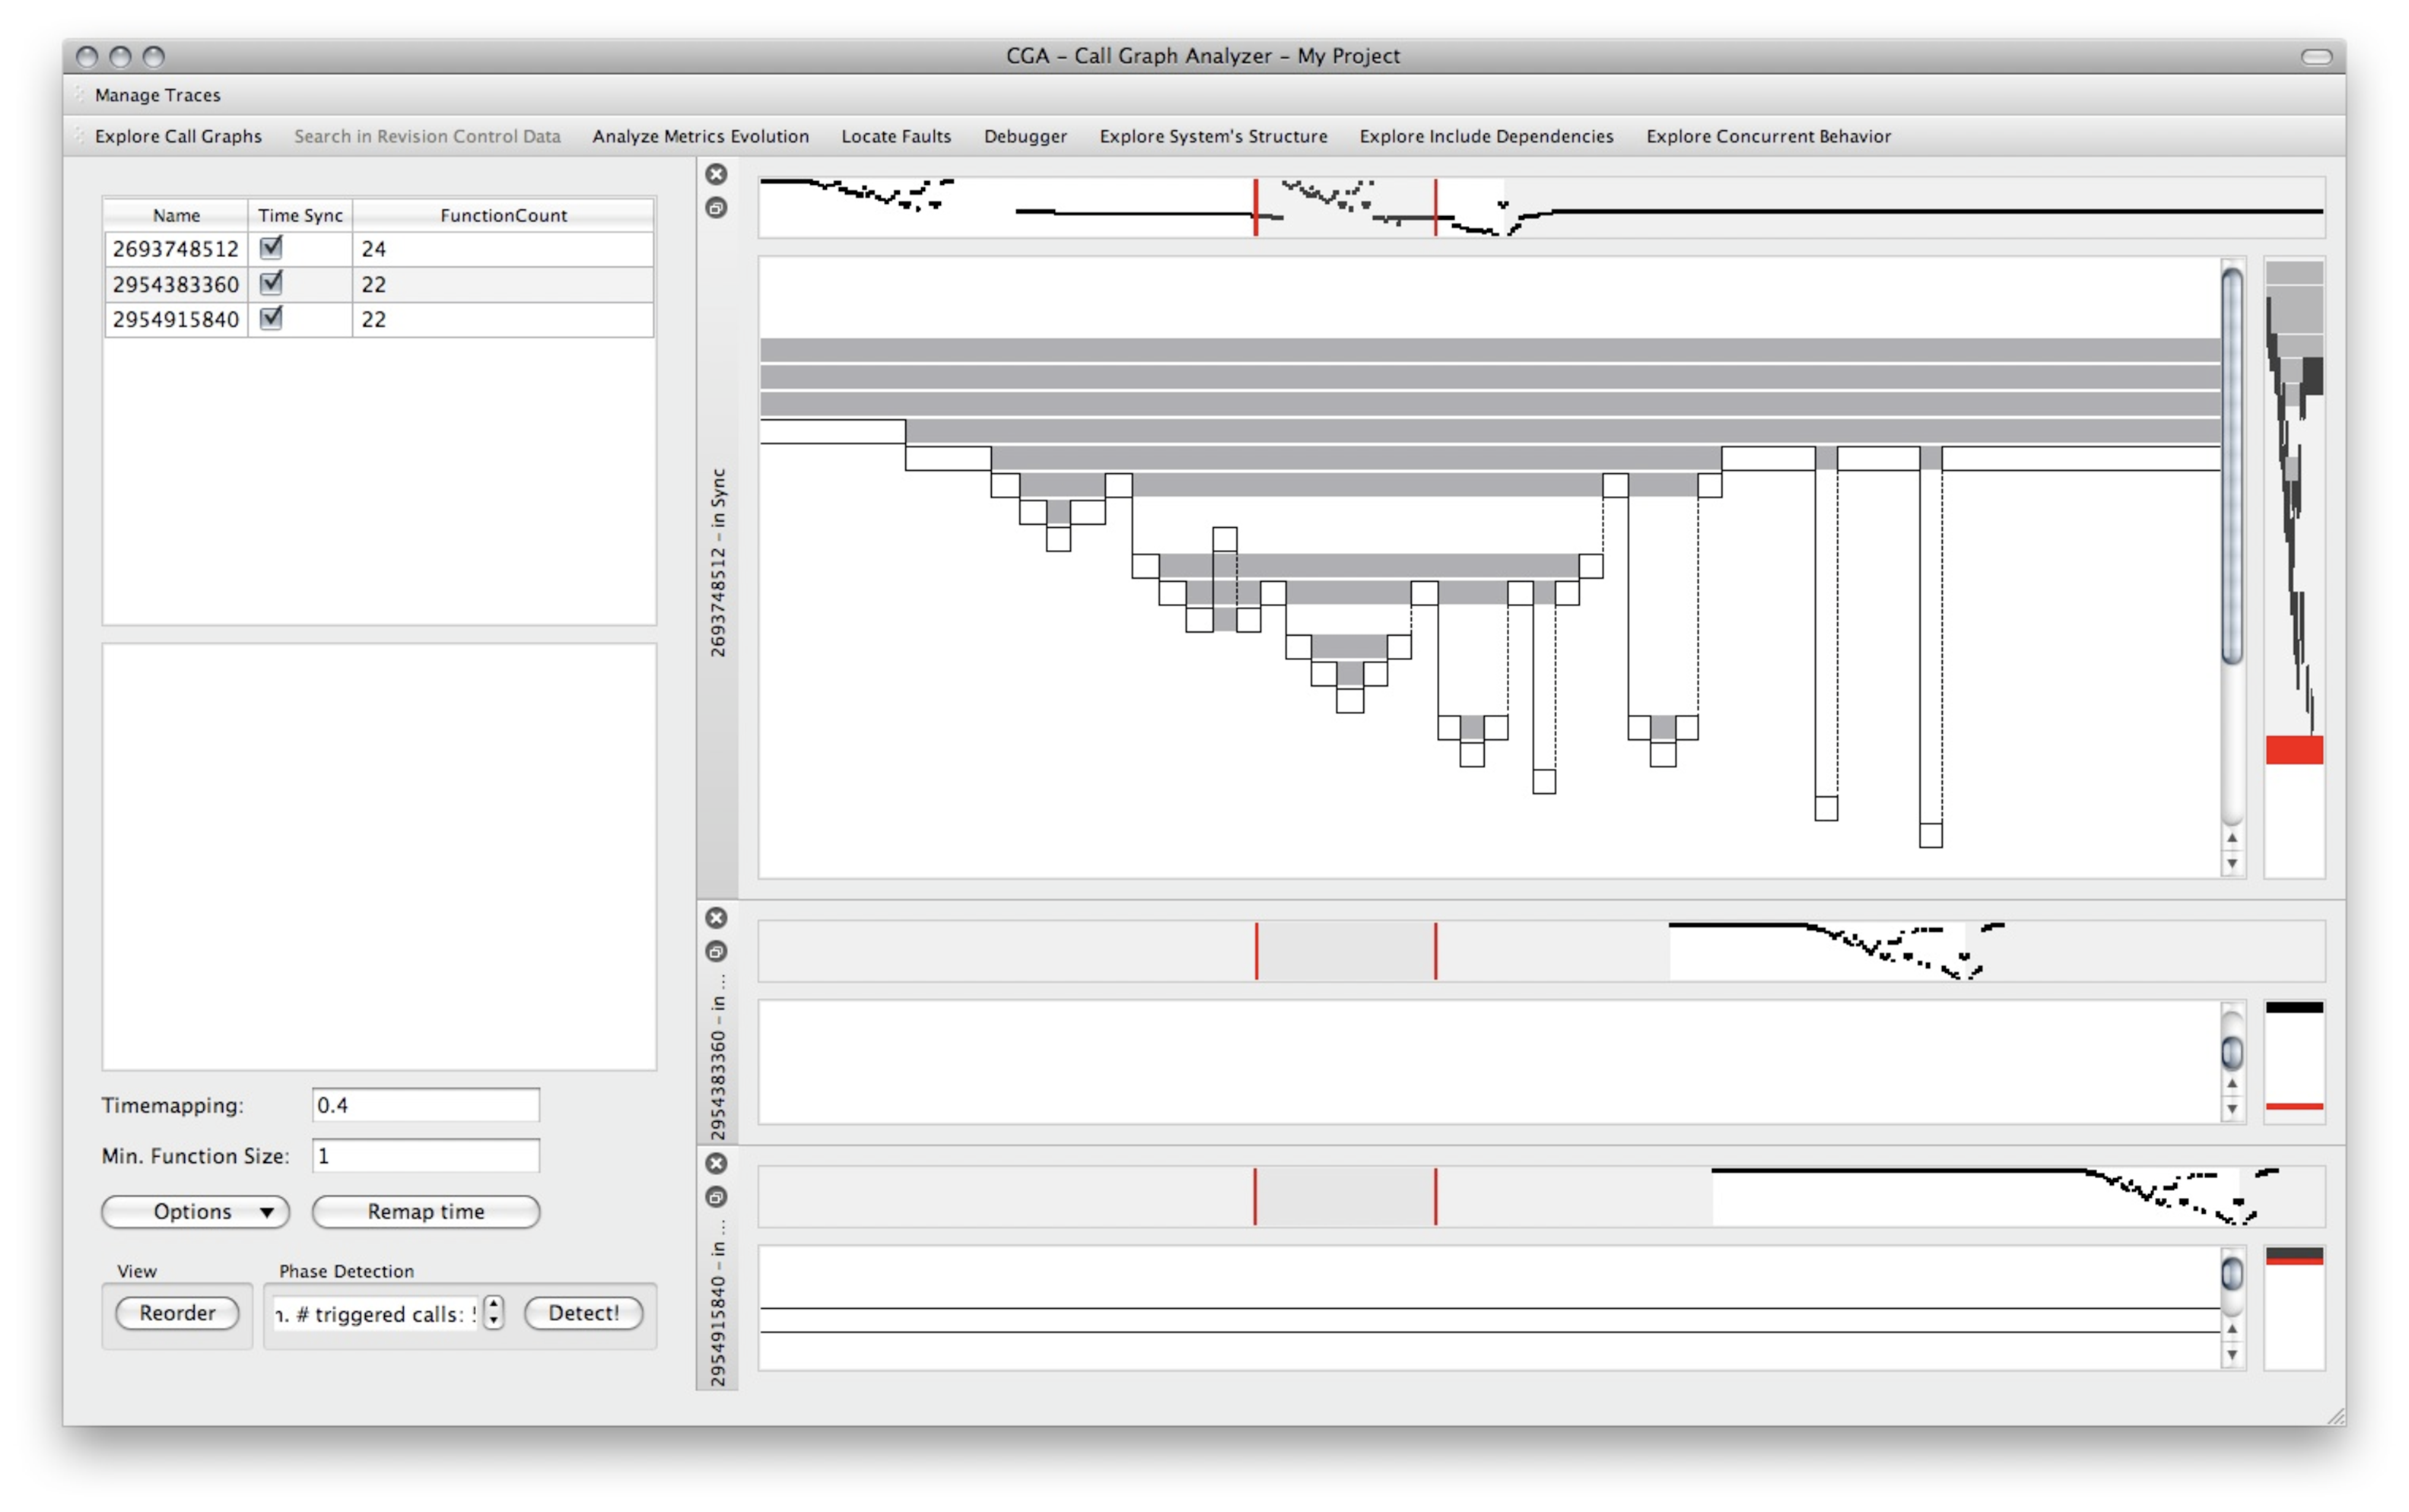
\includegraphics[width=16cm]{images/cga_threads}
\caption{Concurrency Visualisation showing data collected on Unix}\label{fig:cga_threads}
\end{figure}
